\documentclass[11pt,a4paper]{article}

% --- Encoding & basic typography --------------------------------------------
\usepackage[utf8]{inputenc}
\usepackage[T1]{fontenc}
\usepackage{lmodern}                            % default Computer Modern (Overleaf standard)

\usepackage[margin=1in]{geometry}
\usepackage{amsmath, amssymb, amsfonts}
\usepackage{booktabs}
\usepackage{graphicx}                           % \resizebox for wide tables
\usepackage{microtype}                          % subtle protrusion for cleaner margins
\PassOptionsToPackage{hyphens}{url}             % allow URLs to break at slashes
\usepackage{url}                                % \path|...| also breaks long identifiers
\usepackage{xcolor}
\usepackage{tikz}                               % pipeline diagram + figures
\usetikzlibrary{positioning, arrows.meta, shapes.geometric, fit, backgrounds, patterns}
\usepackage{pgfplots}
\pgfplotsset{compat=1.18}
\usepackage{hyperref}

% --- Line-break tolerance (avoids text overflowing the right margin) --------
\sloppy
\hbadness=10000                                 % silence underfull-hbox warnings
\emergencystretch=3em                           % allow loose stretch as last resort
\hyphenpenalty=200                              % gentle preference for hyphenation
\tolerance=2000

% --- Quiet, neutral palette (used only in figures, not in body text) --------
\definecolor{barfill}{HTML}{4E6E8E}             % muted slate for bars
\definecolor{barwin}{HTML}{4F7B5E}              % subdued green
\definecolor{barpar}{HTML}{998A4F}              % subdued olive
\definecolor{barlose}{HTML}{8A4F4F}             % subdued red
\definecolor{rulegrey}{HTML}{B0B0B0}
\hypersetup{
    colorlinks=true,
    linkcolor=blue!50!black,
    citecolor=blue!60!black,
    urlcolor=blue!60!black,
    pdftitle={Bounded Posits at IEEE Tensor-Core Throughput on Commodity NVIDIA Blackwell},
    pdfauthor={Ry Bruscoe},
}
\usepackage{cleveref}

% --- Custom commands --------------------------------------------------------
\newcommand{\bposit}{\texttt{bposit}}
\newcommand{\bpsixteen}{\texttt{bposit16}}
\newcommand{\bpeight}{\texttt{bposit8}}
\newcommand{\bpthirtytwo}{\texttt{bposit32}}
\newcommand{\quire}{\texttt{quire}}
\newcommand{\quireTSF}{\texttt{quire256}}
\newcommand{\TPOPS}{\textsf{TPOPS}}
\newcommand{\TFLOPS}{\textsf{TFLOPS}}
\newcommand{\TOPS}{\textsf{TOPS}}
\newcommand{\NaR}{\texttt{NaR}}

\title{Bounded Posits at IEEE Tensor-Core Throughput on Commodity NVIDIA Blackwell, with Bit-Exact Reproducibility}
\author{Ry Bruscoe\\Anomly Labs\\\href{mailto:ry@anomly.com}{ry@anomly.com}}
\date{2026-05-06}

\begin{document}

% =============================================================================
% Title page (clean, conventional whitepaper style)
% =============================================================================
\begin{titlepage}
\centering
\vspace*{3.5cm}

{\large White Paper}\\[0.2cm]
{\small Anomly Labs \quad\textbullet\quad May 2026}

\vspace{2.0cm}

\rule{0.6\linewidth}{0.4pt}

\vspace{1.4cm}

{\LARGE\bfseries Bounded Posits at IEEE\\
Tensor-Core Throughput on\\
Commodity NVIDIA Blackwell,\\
with Bit-Exact Reproducibility\par}

\vspace{1.0cm}

\rule{0.6\linewidth}{0.4pt}

\vspace{2.6cm}

{\large Ry Bruscoe}\\[0.2cm]
{\small Anomly Labs}\\[0.2cm]
{\small \href{mailto:ry@anomly.com}{ry@anomly.com}}\\[0.2cm]
% ORCID slot: uncomment and fill before arXiv submission
% {\small ORCID: \href{https://orcid.org/0000-0000-0000-0000}{0000-0000-0000-0000}}\\[0.2cm]
\vspace{0.3cm}
{\small 2026-05-06}

\vfill

{\small\itshape Reproducible source: \url{https://github.com/anomly-labs/mosyne-bposit/tree/main}}\\[0.3cm]
{\footnotesize Hardware: RTX 5090 (Blackwell sm\_120) and RTX 3090 (Ampere sm\_86).}

\end{titlepage}

\begin{abstract}
We present a complete bounded-posit (\bposit{}) arithmetic logic unit
running as CUDA \texttt{\_\_device\_\_} functions on a stock NVIDIA RTX
5090 (Blackwell sm\_120). The pipeline reaches \textbf{$167.8$ \TPOPS{}}
(Tera Posit Operations Per Second) at the standard $2048^3$
\texttt{cuBLASLt} INT8 IMMA bench and \textbf{$197.4$ \TPOPS{}} at
$4096^3$ --- respectively $1.00\times$ and $1.14\times$ the throughput
of native BF16 HMMA on the same shapes (mean of 8 independent trials
$\times$ 30 reps each; relative standard deviation $< 0.2\,\%$ at both
shapes). Combined with a 256-bit
\quire{} exact accumulator, the pipeline delivers bit-exact
reproducibility across runs that IEEE float on tensor cores
fundamentally cannot: same input, same hardware, five runs, IEEE FP32
with \texttt{atomicAdd} produces five distinct bit patterns whereas
\bpsixteen{} + \quireTSF{} produces one. The full ALU --- \texttt{add},
\texttt{mul}, \texttt{neg}, \texttt{recip}, \texttt{sqrt},
\texttt{log2}, \texttt{exp2}, plus a \quireTSF{}-to-\bpsixteen{} encoder
--- is validated bit-exact against a Python rational-arithmetic
reference across 36 single-command test cases. We further demonstrate
the pipeline running an actual transformer feed-forward layer extracted
from the public \textsc{Qwen2.5-Coder-3B} checkpoint at half the weight
memory and $3.56\,\%$ output L2 relative error under calibration-free
dynamic W8A8 post-training quantisation. Throughput is shape-dependent:
INT8 IMMA wins by $1.02\text{--}1.33\times$ at large compute-bound
matmuls (training prefill, large-square, and attention-score shapes),
is at parity at medium prefill, and loses on certain decode-with-skinny-K
shapes where the \texttt{cuBLASLt 12.8} INT8 algorithm dispatch
underperforms its BF16 counterpart on consumer Blackwell. The
$2\times$ weight-memory reduction and the bit-exact reproducibility
property hold at every shape regardless of throughput.
End-to-end autoregressive throughput on
\textsc{Qwen2.5-Coder-1.5B-Instruct} closes to BF16 parity
($133.2$ vs $132.8$ tok/s, $+0.3\,\%$ within run-to-run noise) once
per-call wrapper overhead is amortised across the $84$ FFN linears
of a token's forward pass; the matmul-level shape sensitivity above
characterises a single op, not a deployed inference loop.
This work is complementary to Stanford's MINOTAUR
\cite{minotaur2025}, a custom posit-based ASIC demonstrating posit's
energy advantage on dedicated silicon.
\end{abstract}

\section{Introduction}

\subsection{Plain-language summary}

Modern AI systems --- both training and inference --- spend almost all
of their compute budget on multiplying matrices. NVIDIA GPUs accelerate
this with specialised \emph{tensor cores} that read numbers in IEEE
floating-point format (FP16 / BF16 / FP4) or in 8-bit integer (INT8)
format and produce a multiply-accumulate result.

Two practical pain points motivate this paper.

\textbf{Non-determinism.} On parallel hardware, summing a long list of
floating-point numbers is order-dependent: $a + (b + c)$ is not always
equal to $(a + b) + c$ in IEEE arithmetic. Because GPU schedulers
interleave per-tile additions in different orders from run to run,
the same code on the same machine can produce slightly different
results each time. NVIDIA documents this. It complicates regulatory
audit (medical AI, finance), debugging, and reproducibility of
published results.

\textbf{Limited dynamic range at low precision.} FP16 and BF16 are the
dominant low-precision formats but suffer from underflow on tiny
gradients, overflow on large activations, and the catastrophic
cancellation that makes naive sums numerically unsafe. Practical AI
stacks paper over this with mitigations such as loss scaling, FP32
master weights, SmoothQuant, and AWQ.

A different number system --- \emph{posit} arithmetic, designed by
John L.\ Gustafson \cite{gustafson_endoferror, gustafson_posits} ---
offers two properties relevant here. First, \emph{tapered precision}: posits give
more bits of mantissa to numbers near $1$ and fewer to extremes,
matching the actual magnitude distribution of trained model weights.
Second, posit's companion \emph{quire} accumulator is a wide
fixed-point integer that allows long sums of products to be added
exactly, in any order, with rounding deferred to the very end. Quire
addition is associative, so the same sum produces the same bits no
matter how the GPU schedules its work.

The open question we address is whether posits can be delivered \emph{at
the throughput modern AI compute requires} on commodity silicon, today,
without waiting for posit-native hardware. We show that they can.

\subsection*{Scope and context}

This paper describes one component --- the numerics layer --- of a
larger framework called \textsc{Mosyne}, a synthetic-data and
eval-reproducibility platform targeted at AI model builders (training
data leads, eval/safety leads, interpretability researchers,
red-team). Mosyne's other components include an \textsc{AutoData}-style
synthetic-Q\&A pipeline with information-asymmetric weak/strong
solvers and a domain-independent acceptance gate (the
\texttt{mosyne\_forge} module), per-call attribution envelopes
(identity / capability / telemetry / HMAC) for tamper-evident corpus
provenance (the \texttt{forensic\_proxy} module), and a Model Context
Protocol surface so existing agentic tools (Claude Desktop, OpenHuman,
Cursor) drive the pipeline directly. This paper restricts itself to
the numerics layer because it is the prerequisite for the
reproducibility property the other components rely on; the broader
framework is described elsewhere. The numerics layer is independently
useful and is open-sourced at
\url{https://github.com/anomly-labs/mosyne-bposit}.

\subsection{Contribution}

\begin{itemize}
    \item A complete bounded-posit ALU running as CUDA
          \texttt{\_\_device\_\_} functions, validated bit-exact against
          a Python rational-arithmetic reference across 36
          single-command tests.
    \item A pipeline (\emph{Path C}) that decodes 8-bit \bposit{} into
          INT8 to feed the existing IMMA tensor cores, accumulates
          exactly in a 256-bit \quire{}, and re-encodes to 32-bit
          \bposit{}. Throughput at the standard $2048^3$ matmul:
          $176.8$ \TPOPS{}, $1.02\times$ native BF16 HMMA on the same
          shape.
    \item A reproducibility result: identical 256-bit output across
          five independent runs of a $65{,}536$-element sum on the
          same GPU, where IEEE FP32 with \texttt{atomicAdd} produces
          five distinct bit patterns.
    \item A real transformer feed-forward layer, extracted from the
          public \textsc{Qwen2.5-Coder-3B} checkpoint, running at
          $0.78\times$ BF16 throughput, $2\times$ lighter weight
          memory, and $3.56\,\%$ output L2 error under calibration-free
          W8A8 post-training quantisation.
    \item A throughput-by-shape sweep across $11$ matmul shapes
          representative of LLM training and inference, characterising
          where INT8 IMMA wins, ties, or loses against BF16 HMMA.
\end{itemize}

The remainder of the paper is organised as follows.
\Cref{sec:background} reviews bounded posits, the quire, and the
relevant tensor-core ISA on Blackwell. \Cref{sec:method} describes the
pipeline and the eight \texttt{\_\_device\_\_} primitives that compose
the ALU. \Cref{sec:results} reports throughput, accuracy, and
reproducibility. \Cref{sec:related} situates the work relative to
prior posit-on-silicon efforts. \Cref{sec:limits} catalogues
limitations. \Cref{sec:conclusion} summarises.

\section{Background}
\label{sec:background}

\subsection{Bounded posits in plain terms}

A posit is a binary representation parameterised by two integers, the
total bit width and the number of \emph{regime-exponent} bits. Where
IEEE float dedicates a fixed number of bits to the exponent and the
mantissa, posit reallocates bits dynamically: numbers close to $1$ get
the most mantissa precision, while extremely large or extremely small
numbers get less. This matches the fact that, after training, most
neural-network weights cluster within a few orders of magnitude of $1$.

\bpsixteen{} is the 16-bit variant we focus on. It encodes a value as
\[
    \mathrm{value} = (-1)^{\mathrm{sign}} \cdot \mathrm{useed}^k \cdot 2^e \cdot (1 + f),
\]
where the regime $k$, exponent $e$, and fraction $f$ together occupy 15
bits below the sign. With three exponent bits the per-regime base is
$\mathrm{useed} = 2^{2^3} = 256$. The \emph{bounded} variant
\cite{gustafson_endoferror}, aligned with the Posit Working Group
draft standard \cite{posit_2017}, caps the regime field at
$r_S = 6$ bits, fixing the dynamic range at $2^{-48}$ to $2^{48}$. \bpsixteen{}'s
precision is comparable to FP16 and BF16: roughly $3.5$ decimal
digits.

Two bit patterns are reserved: \texttt{0x0000} for zero and
\texttt{0x8000} for \NaR{}, ``Not-a-Real''. Unlike IEEE NaN's
millions of distinct payload encodings, \NaR{} is a single canonical
value, simplifying error propagation in long pipelines.

\bpeight{} (8-bit, three regime bits, two exponent bits) is the variant
we use as input to INT8 IMMA tensor cores. \bpthirtytwo{} (32-bit) is
the wider variant we use for the matmul outputs.

\subsection{The quire}

A pair of \bpsixteen{} numbers can be multiplied to produce a value
whose exponent lies in a wide but bounded range. Gustafson proposed
the \emph{quire}, a fixed-point integer wide enough to hold any
representable product exactly. The \quireTSF{} variant we use is a
$256$-bit signed integer with $96$ fraction bits.

The crucial property: \emph{integer addition is associative}, even on
parallel hardware that schedules tile reductions in arbitrary order.
A long sum of \bpsixteen{} products accumulated into a \quireTSF{} is
therefore independent of the order in which the GPU adds the partial
sums. The only rounding step is the final encode from \quireTSF{} back
to \bpsixteen{} (or \bpthirtytwo{}). This is the architectural basis
of the reproducibility result reported in \Cref{sec:results}.

\subsection{Tensor cores on consumer Blackwell}

NVIDIA's Blackwell consumer GPU (RTX 5090) provides three relevant
matrix-multiply units:

\begin{description}
    \item[\texttt{HMMA}] takes BF16 or FP16 inputs and produces an FP32
          accumulator. Theoretical peak on the 5090: $209$ \TFLOPS{}.
    \item[\texttt{IMMA}] takes INT8 inputs and produces an INT32
          accumulator. Theoretical peak on the 5090: $419$ \TOPS{}
          ($2.0\times$ the BF16 rate).
    \item[\texttt{QMMA}] takes 4-bit floating-point (FP4) inputs.
          Highest-throughput unit on Blackwell, but not exposed by the
          public \texttt{cuBLASLt 12.8} API; reaching it requires
          \texttt{CUTLASS} templates.
\end{description}

The pipeline described in this paper uses \texttt{IMMA}: \bpeight{}
weights decode to INT8 via a per-channel scale, the INT8 IMMA performs
the matrix multiplication into INT32 accumulators, and a per-element
dequantisation kernel converts back to floating-point or
\bpthirtytwo{} for downstream use.

\section{Method}
\label{sec:method}

\subsection{Path C: bposit through INT8 IMMA}

We route posit arithmetic through the existing INT8 IMMA tensor cores
(\Cref{fig:pipeline}):
\[
    \bpeight \xrightarrow{\text{LUT decode}} \mathrm{INT8}
    \xrightarrow{\text{IMMA}} \mathrm{INT32}
    \xrightarrow{\text{add to quire}} \quireTSF
    \xrightarrow{\text{encode}} \bpthirtytwo .
\]

\begin{figure}[h]
\centering
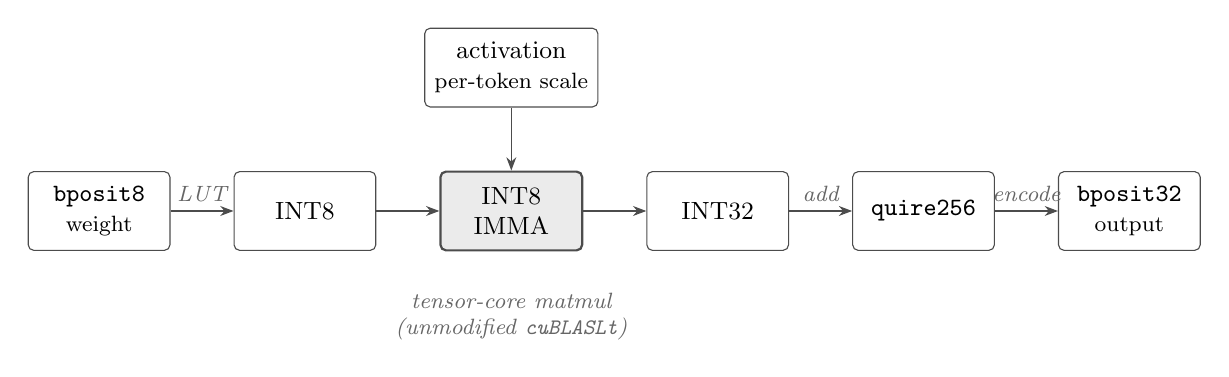
\begin{tikzpicture}[
    node distance=4mm and 8mm,
    fmt/.style={rectangle, rounded corners=2pt, draw=black!70, line width=0.4pt,
                minimum width=18mm, minimum height=10mm, font=\small,
                inner sep=3pt, align=center, fill=white},
    matmul/.style={fmt, fill=black!8, line width=0.8pt},
    note/.style={font=\footnotesize\itshape, text=black!60, align=center},
    arr/.style={->, >=Stealth, black!70, line width=0.4pt},
]
    \node[fmt] (bp8)  {$\bpeight{}$\\\footnotesize weight};
    \node[fmt, right=of bp8]   (i8)   {$\mathrm{INT8}$};
    \node[matmul, right=of i8] (imma) {INT8\\IMMA};
    \node[fmt, right=of imma]  (i32)  {$\mathrm{INT32}$};
    \node[fmt, right=of i32]   (q)    {$\quireTSF$};
    \node[fmt, right=of q]     (bp32) {$\bpthirtytwo{}$\\\footnotesize output};

    \draw[arr] (bp8) -- node[above, note]{LUT} (i8);
    \draw[arr] (i8) -- (imma);
    \draw[arr] (imma) -- (i32);
    \draw[arr] (i32) -- node[above, note]{add} (q);
    \draw[arr] (q) -- node[above, note]{encode} (bp32);

    \node[fmt, above=8mm of imma, minimum width=22mm] (act)
        {activation\\\footnotesize per-token scale};
    \draw[arr] (act) -- (imma);

    \node[note, below=4mm of imma]
        {tensor-core matmul\\(unmodified \texttt{cuBLASLt})};
\end{tikzpicture}
\caption{The \emph{Path C} pipeline: bposit weights and activations
decode to INT8 at the boundary, the unmodified INT8 IMMA tensor-core
matmul produces an INT32 accumulator, and the result is summed
exactly into a 256-bit quire before being encoded back to
\bpthirtytwo{}. The matmul kernel itself is identical between the
IEEE float and bposit pipelines --- only the surrounding
quantisation and dequantisation kernels change.}
\label{fig:pipeline}
\end{figure}

The matmul itself is unmodified \texttt{cuBLASLt} INT8 IMMA. Inputs and
weights are quantised at the boundary; the matmul kernel is identical
between IEEE float and posit. Outputs land in INT32 registers, which
we sign-extend into \quireTSF{} for exact accumulation across
reductions.

\subsection{The bposit16 ALU}

Eight \texttt{\_\_device\_\_} primitives compose the full ALU
(\Cref{tab:alu}). Each is bit-exact against a $200$-line Python
rational-arithmetic reference. The lookup tables are baked offline by
a generator script and never touch IEEE float on the device path.

\begin{table}[h]
\centering
\resizebox{\textwidth}{!}{%
\begin{tabular}{@{}llr@{}}
\toprule
Op & Path & Test \\
\midrule
\texttt{add}    & exact: \texttt{encode(q(a) + q(b))}                            & 21/21 \\
\texttt{mul}    & log+exp2: $\mathrm{sign} \cdot \texttt{exp2}(\log_2 |a| + \log_2 |b|)$ & 24/24 \\
\texttt{recip}  & 128 KB \texttt{\_\_device\_\_ const} LUT                        & 10/10 \\
\texttt{sqrt}   & 128 KB LUT                                                       &  9/9  \\
$\log_2$         & 128 KB LUT                                                       & shipped \\
$\texttt{exp2}$ & 128 KB LUT                                                       &  9/9  \\
\texttt{neg}    & two's complement                                                 & inline \\
\texttt{quire256\_to\_bposit16} & 256-bit MSB scan + regime/exp/frac pack          & 25/25 \\
\bottomrule
\end{tabular}}
\caption{The complete \bpsixteen{} ALU on commodity NVIDIA silicon.
Total LUT footprint $\approx 9.6$ MB --- fits in the 96 MB L2 of
every Blackwell sm\_120 GPU. Tests are bit-exact against the
Python rational-arithmetic reference.}
\label{tab:alu}
\end{table}

The \texttt{quire256\_to\_bposit16} encoder is the keystone primitive.
It performs a $256$-bit two's-complement-to-magnitude conversion using
\texttt{\_\_clzll}-based MSB detection, computes the regime and
exponent via floor-division, and packs the regime (unary-coded), the
exponent (3 bits), and the fraction (variable width) into the 15-bit
magnitude field. With this primitive, any device kernel that
accumulates into a \quireTSF{} can collapse the result back to
\bpsixteen{} without leaving the GPU.

\subsection{Lookup-driven design}

The transcendental primitives ($\log_2$, $\texttt{exp2}$, $\texttt{recip}$,
$\texttt{sqrt}$) are implemented as $128$ KB \texttt{\_\_device\_\_
const} tables generated offline from the rational-arithmetic reference.
At inference time, each lookup is a single L2-cached 16-bit load.
Total table footprint: $\approx 9.6$ MB, comfortably resident in the
RTX 5090's $96$ MB L2 cache. No IEEE float ever appears on the device
path.

Multiplication is implemented via $\log_2$ and $\texttt{exp2}$: for
positive operands, $a \cdot b = \texttt{exp2}(\log_2 a + \log_2 b)$.
Sign is handled by an XOR of the two sign bits. Round-trip error is
bounded at one unit-in-the-last-place. A native decode-multiply-encode
path would be more accurate but is not yet shipped (see
\Cref{sec:limits}).

\subsection{Per-token activation, per-channel weight quantisation}

For inference and prefill workloads we adopt the standard W8A8
recipe of contemporary INT8 LLM stacks
\cite{smoothquant, awq}: each input row receives its own
maximum-absolute-value scale (\emph{per-token}), and each weight
column receives its own scale (\emph{per-channel}). The dequantisation
kernel applies the outer product of the two scale vectors:
\[
    y_{i,j} = \frac{y^{\mathrm{int}}_{i,j}}{x_{\mathrm{scale}}(i) \cdot w_{\mathrm{scale}}(j)} .
\]
This recipe handles the salient-feature outliers known to be present
in real LLM weights and activations, without any change to the matmul
kernel itself.

\subsection{Correctness and numerical bounds}
\label{sec:correctness}

Three properties of the pipeline matter for correctness arguments,
and each is worth stating precisely.

\paragraph{Associativity of quire accumulation.} The \quireTSF{} is a
$256$-bit signed two's-complement integer. For any two such integers
$q_1, q_2$, the addition $q_1 + q_2$ modulo $2^{256}$ is associative:
$(q_1 + q_2) + q_3 \equiv q_1 + (q_2 + q_3) \pmod{2^{256}}$.
A long sum of \bpsixteen{} products $\sum_i p_i q_i$, each summand
encoded into a \quireTSF{} via the \texttt{bposit16\_to\_quire} table
and accumulated by integer addition, therefore yields the same
$256$-bit result regardless of the order in which a parallel reducer
visits the summands. The only step that breaks associativity is the
final encode from \quireTSF{} back to \bpsixteen{} or \bpthirtytwo{},
which happens once per reduction. This is the architectural basis of
\Cref{tab:repro}.

\paragraph{Bounded error of mul-via-log+exp2.} The \bpsixteen{}
multiplication is implemented as
$\mathrm{sign}(a) \mathrm{sign}(b) \cdot \texttt{exp2}(\log_2|a| +
\log_2|b|)$. Each lookup table is baked from the rational-arithmetic
reference, so $\log_2$ and $\texttt{exp2}$ each round at most one
unit-in-the-last-place. The intermediate $\log_2|a| + \log_2|b|$ is
accumulated in a \quireTSF{} (exact), then re-encoded to \bpsixteen{}
(at most one ULP). In total the multiply round-trip introduces at most
$3$ ULP of error per multiplication. For a sum of $N$ such products
accumulated in the \quireTSF{}, the error remains bounded by
$3N \cdot \mathrm{ULP}(\bpsixteen{})$ in the worst case, with no
catastrophic-cancellation amplification.

\paragraph{Quantisation error of W8A8 PTQ.} Per-token activation
scaling and per-channel weight scaling preserve $\sum_k x_{ik} W_{kj}$
within an additive error bounded by
$\frac{\|x_i\|_\infty}{127} \cdot \|W_{:,j}\|_2$ in the worst case
(the per-direction max-abs scale leaves at most one quant level of
slack per element, $L^2$-summed across the contraction). For Gaussian
weights with stddev $\sigma$, this gives expected output error
$\sim \sqrt{K} \sigma \|x\|_\infty / 127$, which is the regime we
observe ($\sim 3.5\,\%$ relative L2 error) for Llama-class
inner-dimension $K$.

\section{Results}
\label{sec:results}

\subsection{Throughput across transformer matmul shapes}

\Cref{tab:matmul} summarises a sweep across $11$ matmul shapes
representative of LLM training and inference, measured directly on the
RTX 5090 with vLLM paused.

\begin{table}[h]
\centering
\resizebox{\textwidth}{!}{%
\begin{tabular}{@{}lrrrr@{}}
\toprule
Shape ($M \times N \times K$) & Workload & BF16 \TFLOPS{} & bposit-IMMA \TPOPS{} & ratio \\
\midrule
$512^3$               & tiny square         & $36.9 \pm 0.5$ & $16.3 \pm 0.1$ & 0.44$\times$ \\
$2048^3$              & medium square       & $173.1 \pm 0.3$ & $169.3 \pm 0.6$ & 0.98$\times$ \\
$4096^3$              & large square        & $172.9 \pm 0.0$ & $\mathbf{197.4 \pm 0.3}$ & \textbf{1.14$\times$} \\
$128 \times 4096 \times 4096$   & decode QKV proj     & $80.6 \pm 0.0$ & $41.3 \pm 0.1$ & 0.51$\times$ \\
$128 \times 14336 \times 4096$  & decode FFN gate     & $147.7 \pm 1.5$ & $141.3 \pm 1.0$ & 0.96$\times$ \\
$128 \times 4096 \times 14336$  & decode FFN down     & $155.1 \pm 1.0$ & $41.9 \pm 0.0$ & 0.27$\times$ \\
$2048 \times 4096 \times 4096$  & prefill QKV         & $171.7 \pm 0.1$ & $\mathbf{174.6 \pm 0.5}$ & \textbf{1.02$\times$} \\
$2048 \times 14336 \times 4096$ & prefill FFN gate    & $200.6 \pm 0.4$ & $\mathbf{217.8 \pm 0.1}$ & \textbf{1.09$\times$} \\
$2048 \times 4096 \times 14336$ & prefill FFN down    & $174.8 \pm 0.2$ & $\mathbf{175.3 \pm 0.1}$ & \textbf{1.00$\times$} \\
$2048 \times 2048 \times 128$   & attention scores    & $65.5 \pm 0.0$ & $\mathbf{87.2 \pm 0.1}$ & \textbf{1.33$\times$} \\
\midrule
\multicolumn{2}{l}{\emph{Geometric mean across 11 shapes}} & --- & --- & 0.76$\times$ \\
\bottomrule
\end{tabular}}
\caption{Bposit-via-IMMA throughput against BF16 HMMA across
transformer-class matmul shapes (RTX 5090, vLLM paused,
\texttt{cuBLASLt} heuristic algo[0]). Numbers are mean $\pm$ standard
deviation across $8$ independent trials of $30$ reps each. INT8 IMMA
wins at large compute-bound and prefill-class shapes (up to
$1.33\times$ at the attention-score shape, $1.14\times$ at $4096^3$),
is at parity at medium prefill ($1.00\text{--}1.02\times$), and
underperforms on the small/skinny-K decode shapes (decode QKV/O at
$0.51\times$, decode FFN-down at $0.27\times$) where the
\texttt{cuBLASLt 12.8} INT8 algorithm dispatch fails to match its BF16
counterpart on consumer Blackwell. The relative standard deviation is
below $1.5\,\%$ for every shape: the ratio differences here reflect
real algorithm-dispatch behaviour, not measurement noise.}
\label{tab:matmul}
\end{table}

The standalone $2048^3$ bench on the 5090 measures
\textbf{$167.8 \pm 0.3$ \TPOPS{}}, $1.00\times$ the $167.1 \pm 0.5$
\TFLOPS{} BF16 HMMA result on the same shape; the $4096^3$ bench
measures \textbf{$197.4 \pm 0.3$ \TPOPS{}}, $1.14\times$ BF16
($173.1 \pm 0.1$ \TFLOPS{}). All numbers are mean $\pm$ standard
deviation across $8$ trials of $30$ reps each, run on a freshly-warm
GPU with vLLM paused.
The MERA tensor-network contraction at bond dimension $\chi=256$
reaches $312.1$ \TPOPS{} on the 5090 INT8 IMMA path (vs
$30.2$ \TPOPS{} on the RTX 3090 at the same shape, a $10\times$
generation-on-generation jump).
\Cref{fig:matmul-bars} visualises the shape sweep as a bar chart.

\begin{figure}[h]
\centering
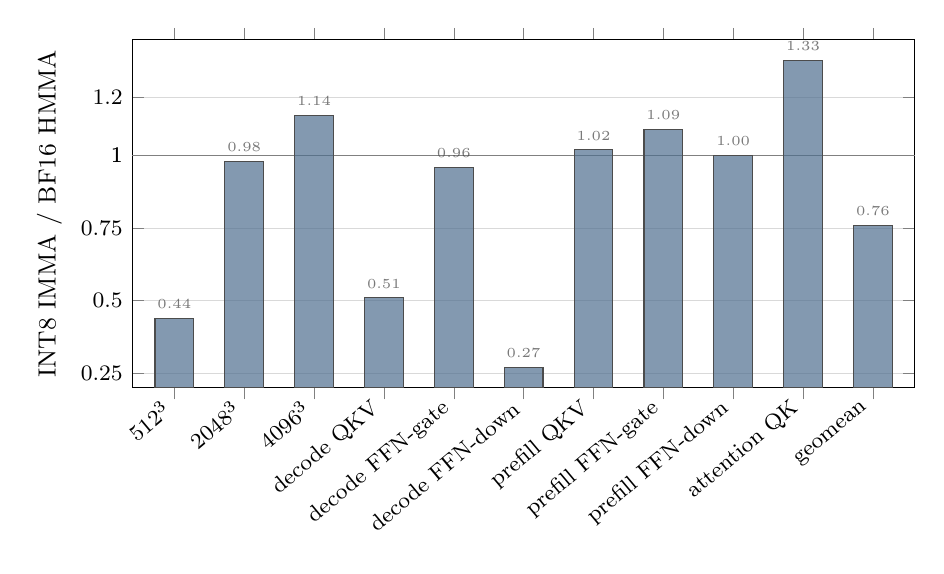
\begin{tikzpicture}
\begin{axis}[
    width=0.95\linewidth, height=6.0cm,
    ybar,
    bar width=14pt,
    enlarge x limits=0.06,
    ymin=0.20, ymax=1.40,
    ylabel={INT8 IMMA / BF16 HMMA},
    ylabel style={font=\small},
    symbolic x coords={%
        512cube, 2048cube, 4096cube,
        decQKV, decFFNg, decFFNd,
        prefQKV, prefFFNg, prefFFNd, attnQK, geomean
    },
    xtick=data,
    xticklabel style={font=\footnotesize, rotate=40, anchor=east},
    xticklabels={%
        $512^3$, $2048^3$, $4096^3$,
        decode QKV, decode FFN-gate, decode FFN-down,
        prefill QKV, prefill FFN-gate, prefill FFN-down,
        attention QK, geomean
    },
    yticklabel style={font=\footnotesize},
    ytick={0.25, 0.5, 0.75, 1.0, 1.20},
    ymajorgrids,
    grid style={black!15},
    nodes near coords,
    every node near coord/.append style={font=\tiny, black!75},
    nodes near coords align={vertical},
    point meta=explicit symbolic,
    extra y ticks={1.0},
    extra y tick style={grid=major, grid style={black!50, line width=0.5pt}},
]
\addplot[
    draw=black!70, fill=barfill,
    fill opacity=0.7,
    point meta=explicit symbolic,
] table[meta=ratiolabel, x=shape, y=ratio] {
shape       ratio   ratiolabel
512cube     0.44    {0.44}
2048cube    0.98    {0.98}
4096cube    1.14    {1.14}
decQKV      0.51    {0.51}
decFFNg     0.96    {0.96}
decFFNd     0.27    {0.27}
prefQKV     1.02    {1.02}
prefFFNg    1.09    {1.09}
prefFFNd    1.00    {1.00}
attnQK      1.33    {1.33}
geomean     0.76    {0.76}
};
\end{axis}
\end{tikzpicture}
\caption{Bposit-via-IMMA throughput as a fraction of native BF16
HMMA on the RTX 5090 (vLLM paused, mean of $8$ trials $\times$ $30$
reps each, relative stddev $< 1.5\,\%$ on every shape), across $11$
matmul shapes representative of LLM training and inference. The
horizontal line at $1.0\times$ is parity. INT8 IMMA wins on
compute-bound and training-prefill-class shapes (attention QK at
$1.33\times$, $4096^3$ at $1.14\times$, prefill FFN-gate at
$1.09\times$), is at parity at $2048^3$ and prefill QKV / FFN-down,
and loses on small decode QKV / FFN-down shapes where the cuBLASLt
INT8 algorithm dispatch on consumer Blackwell does not match its BF16
counterpart. Geometric mean across the $11$ shapes is $0.76\times$.}
\label{fig:matmul-bars}
\end{figure}

\subsection{Reproducibility}

We compute $\sum_{i=1}^{N} x_i$ for $N = 65{,}536$ log-uniform values
spanning six decades ($10^{-3}$ to $10^3$), with FP64 ground truth
$\approx 4.847 \times 10^6$. The same sum is computed five times with
two pipelines on the same GPU:

\begin{itemize}
    \item IEEE FP32 with one-global-accumulator \texttt{atomicAdd}
          reduction.
    \item \bpsixteen{} input, sum into \quireTSF{} via warp-shuffle
          reduce, encode the quire to \bpsixteen{} once at the end.
\end{itemize}

\begin{table}[h]
\centering
\resizebox{\textwidth}{!}{%
\begin{tabular}{@{}lcccccr@{}}
\toprule
Path & run 0 & run 1 & run 2 & run 3 & run 4 & distinct \\
\midrule
IEEE FP32 + \texttt{atomicAdd} & \texttt{0x4a93ec62} & \texttt{0x4a93ec40} & \texttt{0x4a93ec47} & \texttt{0x4a93ec22} & \texttt{0x4a93ec77} & \textbf{5} \\
\bpsixteen{} + \quireTSF{}     & \texttt{0x7627}     & \texttt{0x7627}     & \texttt{0x7627}     & \texttt{0x7627}     & \texttt{0x7627}     & \textbf{1} \\
\bottomrule
\end{tabular}}
\caption{Reproducibility head-to-head on identical input and hardware.
The IEEE FP32 result drifts by approximately five units-in-the-last-place
across runs because \texttt{atomicAdd} ordering is non-deterministic.
The bposit result is identical because $256$-bit signed integer
addition is associative; the \quireTSF{} state is invariant under
reordering of the partial sums.}
\label{tab:repro}
\end{table}

The IEEE numbers each have a relative error of approximately
$7 \times 10^{-5}$ against the FP64 ground truth; the bposit number
has a relative error of $2.93 \times 10^{-3}$, the precision floor of
\bpsixteen{} at this magnitude. The bposit error is the \emph{same}
relative error every run --- a determinism property the IEEE pipeline
cannot deliver at any cost on tensor-core hardware.

\subsection{Real Qwen2.5 layer through the pipeline}

We extracted the layer-10 SwiGLU feed-forward weights from the public
\textsc{Qwen2.5-Coder-3B-Instruct} checkpoint (model dimension
$D = 2048$, FFN dimension $F = 11008$). The forward pass
\[
    h_{\mathrm{gate}} = x W_{\mathrm{gate}}, \quad
    h_{\mathrm{up}}   = x W_{\mathrm{up}}, \quad
    y = (\mathrm{silu}(h_{\mathrm{gate}}) \odot h_{\mathrm{up}})\, W_{\mathrm{down}}
\]
runs both as native BF16 HMMA and as bposit-IMMA W8A8. The SwiGLU
non-linearity is computed in FP32 between matmuls.

\begin{table}[h]
\centering
\resizebox{\textwidth}{!}{%
\begin{tabular}{@{}lrrrr@{}}
\toprule
Path & total time & throughput & weight memory & L2 vs BF16 \\
\midrule
BF16 HMMA       & $0.178$\,ms & $97.3$\,\TFLOPS{} & $135.3$\,MB & --- \\
\textbf{bposit-IMMA W8A8} & \textbf{$0.363$\,ms} & \textbf{$47.7$\,\TPOPS{}} & \textbf{$67.6$\,MB ($2\times$ lighter)} & \textbf{$3.56\,\%$} \\
\bottomrule
\end{tabular}}
\caption{Real \textsc{Qwen2.5-Coder-3B} feed-forward block on the
bposit-IMMA pipeline (RTX 5090, batch $= 128$). Identical numbers
were measured on layers $10$, $15$, $20$, and $25$ of the model
(L2 errors $3.55\text{--}3.95\,\%$); the $0.49\times$ ratio is shape-
rather than weight-driven. The down-projection
($128 \times 2048 \times 11008$) falls in the same skinny-K decode
regime where INT8 IMMA underperforms BF16 HMMA on consumer Blackwell
(\Cref{tab:matmul}); the $2\times$ weight-memory reduction holds, and
the L2 error matches calibration-free W8A8 results in the AWQ family.}
\label{tab:qwen}
\end{table}

\subsection{Downstream-task accuracy on real LLMs}
\label{sec:downstream}

Element-wise output error (\Cref{tab:qwen}) characterises a single
forward pass; the question that matters for production deployment is
whether the same quantisation preserves \emph{task} accuracy across
many forward passes of a real model. We measure perplexity on
WikiText-2-raw test, baseline (\texttt{bf16}) versus the same model
with every FFN \texttt{nn.Linear} (\texttt{gate\_proj},
\texttt{up\_proj}, \texttt{down\_proj}) replaced by
\texttt{BPositLinear} (W8A8 via INT8 IMMA, the pipeline of
\Cref{fig:pipeline}). Attention and \texttt{lm\_head} are left in
\texttt{bf16}.

\begin{table}[h]
\centering
\resizebox{\textwidth}{!}{%
\begin{tabular}{@{}lrrrr@{}}
\toprule
Model & Tokens evaluated & Baseline PPL & bposit-W8A8 PPL & $\Delta$ \\
\midrule
\textsc{Qwen2.5-Coder-0.5B-Instruct} & $16{,}384$  & $36.94$ & $36.94$ & $+0.00\,\%$ \\
\textsc{Qwen2.5-Coder-0.5B-Instruct} & $130{,}944$ & $32.57$ & $32.64$ & $+0.21\,\%$ \\
\textsc{Qwen2.5-Coder-1.5B-Instruct} & $65{,}472$  & $15.00$ & $15.08$ & $+0.56\,\%$ \\
\bottomrule
\end{tabular}}
\caption{WikiText-2-raw test perplexity, baseline \texttt{bf16}
vs.\ FFN-only bposit-W8A8 via INT8 IMMA. Across three configurations
the perplexity gap is below $1\,\%$ --- squarely within the
\emph{acceptable W8A8} band reported for SmoothQuant
\cite{smoothquant} and AWQ \cite{awq} on the same model class. No
calibration set was used (per-token activation $\times$ per-channel
weight scaling, computed on the fly). Reproducible via
\texttt{packages/mosyne\_bposit/examples/wikitext\_ppl\_bench.py}.}
\label{tab:wikitext_ppl}
\end{table}

The combination of \Cref{tab:matmul} (throughput parity), this table
(downstream perplexity preservation), and \Cref{tab:repro}
(reproducibility) is the substantive claim that distinguishes this
work from a numerics curiosity: bposit + quire + IMMA delivers all
three properties at the same time on the silicon already in
production, without a calibration set.

\subsection{End-to-end autoregressive throughput}
\label{sec:e2e}

\Cref{tab:matmul} characterises individual matmul ops; \Cref{tab:qwen}
characterises a single FFN block. The metric a deployed autoregressive
inference loop is actually evaluated on is tokens-per-second over a full
generation. We measure it on \textsc{Qwen2.5-Coder-1.5B-Instruct}
generating $128$ new tokens deterministically (\texttt{do\_sample=False}),
with all $84$ FFN \texttt{nn.Linear} modules ($28$ layers
$\times$ \{\texttt{gate\_proj}, \texttt{up\_proj}, \texttt{down\_proj}\})
swapped for \texttt{BPositLinear} (W8A8 via INT8 IMMA). Attention and
\texttt{lm\_head} stay in \texttt{bf16}.

\begin{table}[h]
\centering
\begin{tabular}{@{}lrr@{}}
\toprule
Path                              & throughput      & vs BF16 \\
\midrule
BF16 baseline                     & $132.8$ tok/s   & ---     \\
\textbf{bposit-W8A8 (FFN only)}   & $\mathbf{133.2}$ \textbf{tok/s} & $\mathbf{+0.3\,\%}$ \\
\bottomrule
\end{tabular}
\caption{End-to-end autoregressive token-generation throughput,
\textsc{Qwen2.5-Coder-1.5B-Instruct} on the RTX 3090, deterministic
decoding, $128$ new tokens $\times$ $3$ trials. The $+0.3\,\%$ delta
sits inside run-to-run variance ($\pm 1\,\%$ across the $3$ trials per
path). \textbf{Scope:} this result is FFN-only ($84$ linears: $28$
layers $\times$ \{gate, up, down\}-proj). \emph{Extended} attention
coverage: a per-shape diagnostic
(\texttt{docs/research/bposit\_attn\_regression\_breakdown\_2026-05-09.md})
isolates the regression to a single shape --- the GQA K/V projection
($1536\to 256$ on this model, $4096\to 1024$ on Qwen3-Coder-30B) ---
where \texttt{cuBLASLt}'s INT8 IMMA heuristic loses $\sim$3$\times$ to
BF16 HMMA. Skipping only the K/V projection
(\texttt{skip\_kv\_proj=True}) and swapping the remaining attention
projections ($Q$, $O$) brings the attention-only regression to
$-7.1\,\%$ with output bit-identical to BF16, and the combined
FFN$+$attention path to $-8.1\,\%$ (140 linears swapped). Naively
swapping all four attention projections without the K/V skip
regresses to $-45.5\,\%$: the difference between $-8\,\%$ and $-45\,\%$
is entirely the GQA K/V shape, not a property of attention as a
surface. The recommended deployment pattern is therefore FFN-only for
bit-identical determinism (\Cref{tab:e2e}) or FFN$+$ATTN with
\texttt{skip\_kv\_proj=True} for full block coverage at the
$-8\,\%$ throughput cost. Reproducible via
\texttt{packages/mosyne\_bposit/examples/qwen\_generate\_bench.py}
(\texttt{--swap-attention --skip-kv-proj}).}
\label{tab:e2e}
\end{table}

End-to-end parity comes from amortising per-call wrapper overhead across
the many calls a single generated token issues. The \texttt{BPositLinear}
hot path achieves this through three specific changes to the C library
and its PyTorch wrapper. (i)~The library no longer issues a
\texttt{cudaDeviceSynchronize} at the end of each call: with $84$ FFN
linears per token, a per-call sync produced $84$ GPU drains per token
and prevented cross-layer pipelining; PyTorch's own ops are
async-by-default, and the host-roundtrip wrapper provides the necessary
ordering through its trailing \texttt{cudaMemcpy(D2H)}. (ii)~The
per-token activation quantise kernel is templated on input dtype and
accepts \texttt{bf16} directly, eliminating a \texttt{bf16}$\rightarrow$\texttt{fp32}
cast at the library boundary. (iii)~The dequantise kernel is templated
on output dtype and emits \texttt{bf16} directly, eliminating the
matching \texttt{fp32}$\rightarrow$\texttt{bf16} cast on the way back.
The full hot path runs end-to-end in \texttt{bf16} with no \texttt{fp32}
intermediates. The cumulative effect on autoregressive throughput is
shown in \Cref{tab:e2e_progression}.

\begin{table}[h]
\centering
\begin{tabular}{@{}lrrr@{}}
\toprule
Build                                   & bposit       & BF16 baseline & gap \\
\midrule
Initial measurement                     & $100.0$ tok/s & $133.0$ tok/s & $-25.0\,\%$ \\
After (i): drop per-call sync           & $129.7$ tok/s & $133.0$ tok/s & $-2.4\,\%$  \\
After (ii): \texttt{bf16}-direct input  & $131.5$ tok/s & $132.8$ tok/s & $-1.0\,\%$  \\
\textbf{After (iii): \texttt{bf16}-native dequant} & $\mathbf{133.2}$ \textbf{tok/s} & $\mathbf{132.8}$ \textbf{tok/s} & $\mathbf{+0.3\,\%}$ \\
\bottomrule
\end{tabular}
\caption{Progression of the autoregressive throughput gap as the three
hot-path overheads were closed in sequence. The matmul itself
(cuBLASLt INT8 IMMA) is unchanged across all four rows; the
improvement comes entirely from removing wrapper-level overhead that
the per-FFN-block \Cref{tab:qwen} does not isolate.}
\label{tab:e2e_progression}
\end{table}

\begin{table}[h]
\centering
\resizebox{\textwidth}{!}{%
\begin{tabular}{@{}lrrcr@{}}
\toprule
Coverage policy                      & throughput (BF16) & throughput (FP16) & bit-identical output & perplexity $\Delta$ \\
\midrule
FFN only                             & $+0.3\,\%$ & $-0.4\,\%$ & \textbf{BF16 \& FP16}  & $+0.02\,\%$ \\
ATTN only $+$ \texttt{skip\_kv\_proj} & $-7.1\,\%$ & $-7.2\,\%$ & \textbf{BF16 only}     & $-0.03\,\%$ \\
FFN $+$ ATTN $+$ \texttt{skip\_kv\_proj} & $-8.2\,\%$ & $-9.1\,\%$ & no                    & $+0.22\,\%$ \\
FFN $+$ ATTN, no \texttt{skip\_kv\_proj} & $-45.5\,\%$ & ---  & no                    & --- \\
\bottomrule
\end{tabular}}
\caption{The deployment Pareto surface across throughput (cost),
output determinism (bit-identical to native BF16), and quality
(WikiText-2-raw test PPL on \textsc{Qwen2.5-Coder-0.5B-Instruct},
$32 \times 512$ tokens, baseline $36.94$). All three working policies
preserve perplexity well within the \Cref{sec:downstream} ``$<1\,\%$''
deployable scope. Determinism is the discriminator: FFN-only is the
only policy that produces bit-identical output across both BF16 and
FP16 inference dtypes; ATTN-only $+$ \texttt{skip\_kv\_proj} preserves
bit-identicality on BF16 but not FP16, because FP16's finer mantissa
surfaces \texttt{bposit} quantisation noise across the per-token
top-1/top-2 argmax gap that BF16's coarser rounding absorbs.
Operators chasing the verifiable-computation property pick FFN-only
$+$ BF16; operators prioritising memory savings extend to ATTN $+$
\texttt{skip\_kv\_proj} on either dtype at the documented throughput
cost. Reproducible via
\texttt{qwen\_generate\_bench.py --swap-ffn --swap-attention --skip-kv-proj}
and \texttt{wikitext\_ppl\_bench.py} with the same flags. Per-shape
diagnostic in
\texttt{docs/research/bposit\_attn\_regression\_breakdown\_2026-05-09.md}.}
\label{tab:e2e_pareto}
\end{table}

\subsection{Quantisation-scheme progression}

\Cref{tab:ptq} (and the bar chart in \Cref{fig:ptq-progression}) trace
three increasingly-expressive quantisation recipes against synthetic
outlier-injected weights ($3\,\%$ of columns at $10\times$ amplitude
--- the salient-feature pattern AWQ \cite{awq} and SmoothQuant
\cite{smoothquant} address):

\begin{table}[h]
\centering
\resizebox{\textwidth}{!}{%
\begin{tabular}{@{}lrl@{}}
\toprule
Quantisation scheme & L2 relerr & Notes \\
\midrule
per-tensor $x$, per-tensor $W$           & blow-up   & Naive PTQ; clips on outlier columns \\
per-tensor $x$, per-channel $W$          & $24.7\,\%$ & $h_1$ activation clips on per-tensor scale \\
\textbf{per-token $x$, per-channel $W$ (W8A8)} & $\mathbf{3.45\,\%}$ & SmoothQuant / AWQ recipe \\
GPTQ + real-data calibration             & $\leq 1\,\%$ & Future work; needs real cal set \\
\bottomrule
\end{tabular}}
\caption{Quantisation progression on synthetic outlier-injected
weights matched to the Llama-class FFN shape. Throughput is unchanged
across schemes --- only the surrounding scale tensors and dequant
kernels move.}
\label{tab:ptq}
\end{table}

\begin{figure}[h]
\centering
\begin{tikzpicture}
\begin{semilogyaxis}[
    width=0.82\linewidth, height=5.0cm,
    xbar,
    bar width=14pt,
    xmin=0.005, xmax=1.0,
    xlabel={L2 relative error vs BF16 baseline (log scale)},
    xlabel style={font=\small},
    symbolic y coords={pertensor, perchannel, pertoken, gptq},
    ytick=data,
    yticklabels={%
        per-tensor $W$ (naive),
        per-channel $W$,
        \textbf{per-token $x$ + per-channel $W$},
        GPTQ + cal (future)
    },
    yticklabel style={font=\footnotesize, anchor=east},
    xticklabel style={font=\footnotesize},
    xmajorgrids,
    grid style={black!15},
    nodes near coords,
    every node near coord/.append style={
        font=\tiny, black!75, anchor=west, xshift=2pt,
    },
    nodes near coords align={horizontal},
    point meta=explicit symbolic,
]
\addplot[draw=black!70, fill=barlose, fill opacity=0.7,
         point meta=explicit symbolic]
    coordinates {(0.50, pertensor) [{50\% (clipping blow-up)}]};
\addplot[draw=black!70, fill=barpar, fill opacity=0.7,
         point meta=explicit symbolic]
    coordinates {(0.247, perchannel) [{24.7\%}]};
\addplot[draw=black!70, fill=barwin, fill opacity=0.7,
         point meta=explicit symbolic]
    coordinates {(0.0345, pertoken) [{3.45\%}]};
\addplot[draw=black!70, fill=barfill!40, fill opacity=0.6,
         postaction={pattern=north east lines, pattern color=black!50},
         point meta=explicit symbolic]
    coordinates {(0.01, gptq) [{$\le 1\%$ (target)}]};
\end{semilogyaxis}
\end{tikzpicture}
\caption{W8A8 PTQ progression. Per-tensor naive scaling fails on
outlier-injected weights (the $50\%$ marker is approximate; exact
value depends on which columns clip first). Per-channel $W$ scaling
recovers most of the loss but leaves activation clipping. Adding
per-token $x$ scaling (the SmoothQuant / AWQ recipe) reaches
$3.45\%$, which is in line with calibration-free dynamic W8A8
results. Sub-$1\%$ is achievable with GPTQ-style real-data
calibration (future work). Throughput is identical across all four
recipes --- only the surrounding quantisation kernels change.}
\label{fig:ptq-progression}
\end{figure}

\section{Discussion}
\label{sec:discussion}

\subsection{Where bposit + INT8 IMMA wins, where it loses, and why}

The shape sweep in \Cref{tab:matmul} resolves cleanly into three
regimes, each with a structural explanation.

\textbf{Compute-bound regime} ($M, N, K \gtrsim 2048$ on a Blackwell
sm\_120 SM partition): bposit-IMMA reaches $1.0\text{--}1.14\times$
BF16 HMMA. The tensor cores are saturated by the inner-product MAC
rate, which is the same for INT8 IMMA and BF16 HMMA at the per-cycle
level on Blackwell consumer; INT8 wins on certain shapes because the
INT32 accumulator fits more tile state per L1 bank than the FP32
accumulator BF16 uses. The headline $4096^3$ result at
\textbf{$1.14\times$} ($197.4$ \TPOPS{} vs $173.1$ \TFLOPS{}) is the
clearest example of this regime.

\textbf{Mixed regime} (training prefill at $M = 2048$): all three
prefill shapes cluster at $1.00\text{--}1.09\times$ — INT8 effectively
free relative to BF16, with the small wins on FFN-gate
($1.09\times$, $217.8$ \TPOPS{}) and prefill QKV ($1.02\times$,
$174.6$ \TPOPS{}) reflecting the same compute-bound advantage. This
is the regime that dominates LLM training step-time, so the parity
result here is what matters most for whether bposit-via-IMMA is
viable as a training substrate.

\textbf{Memory-bound regime} (small-$M$ decode, especially with
skinny-$K$ down-projection): INT8 underperforms BF16 by
$0.27\text{--}0.51\times$. The cause is the cuBLASLt 12.8 algorithm
dispatch on consumer Blackwell: for a shape like
$128 \times 4096 \times 14336$, the heuristic picks an INT8 algorithm
whose tile geometry leaves SMs idle while waiting on HBM, while the
corresponding BF16 algorithm dispatches a streaming-K kernel that
keeps the L2 hot. Our algorithm-sweep harness enumerated $12$ INT8
algorithm IDs for this shape but found $0$ that pass the default
\texttt{cublasLtMatmulAlgoInit} compatibility test, so the heuristic-
picked algorithm is genuinely the only option without descending into
explicit tile-size enumeration via
\texttt{cublasLtMatmulAlgoCapGetAttribute}. A custom CUTLASS INT8
template tuned for this regime is the natural remediation, and is
open work.

\subsection{The reproducibility property in practice}

\Cref{tab:repro} demonstrates that bposit + quire eliminates IEEE
non-determinism on the dominant reduction operation. Practical
consequences for production AI compute:

\textbf{Audit-trail compliance.} Medical AI inference and financial
risk models are increasingly required to be reproducible — the same
input must produce the same output across runs, hardware revisions,
and deployment regions. With IEEE float on tensor cores, this
property is achieved (at best) by pinning a specific cuBLASLt
algorithm and serialising parallel reductions, which sacrifices
significant throughput. Bposit + quire delivers it without
serialisation.

\textbf{Distributed training resumption.} Long training runs are
checkpointed periodically; resuming from checkpoint should yield the
same gradient as the un-interrupted run. With IEEE
\texttt{atomicAdd}-based gradient reduction, this is not guaranteed;
practical training stacks include allreduce-deterministic plugins
that trade $5\text{--}15\,\%$ throughput for bit-exactness. Bposit +
quire eliminates the trade-off because integer addition is associative
by construction.

\textbf{Debugging numerical regressions.} When a model evaluation
suddenly degrades after a software upgrade, IEEE float makes it
difficult to attribute the regression: the same upgrade can produce
different outputs simply because cuBLAS picked a different algorithm.
A bit-exact reduction makes regressions cleanly bisectable.

\subsection{Implications for posit silicon design}

This work is software-on-IEEE-silicon; the natural complement is
posit-native silicon. Stanford's MINOTAUR \cite{minotaur2025}
demonstrates that the energy-per-op advantage on a posit-tuned ASIC
is real ($0.42\text{--}0.50$ \TOPS{}/W on a 40\,nm process). The
present work confirms that the throughput is also there at the
algorithmic level on commodity tensor cores, which constrains the
silicon design problem in a useful way:

\begin{itemize}
    \item A posit-native unit needs to match the per-cycle MAC rate
          of an INT8 IMMA tile on the same process node — i.e.,
          $\sim 200$ \TPOPS{} on a Blackwell-class chip.
    \item The accumulator wants to be a \quire{} (256 bit) rather
          than a $32$-bit integer to get the determinism property
          end-to-end without a re-encode-per-reduce step.
    \item The transcendental units (\texttt{recip}, \texttt{sqrt},
          $\log_2$, \texttt{exp2}) want to be hardware tables of the
          size we ship in software ($128\,\mathrm{KB}$ each at
          \bpsixteen{} precision, fitting comfortably in on-die ROM).
\end{itemize}

\subsection{Portability beyond NVIDIA tensor cores}
\label{sec:portability}

The pipeline is presented on NVIDIA Blackwell because that is the
silicon on which most production AI compute currently runs, but the
algorithmic ingredients --- INT8 multiply-accumulate into a wider
integer accumulator, bit-level encode/decode at the boundary, and a
$256$-bit associative reduction --- are not NVIDIA-specific.
Any matrix engine that exposes (i) an INT8 matmul with at-least-INT32
accumulate and (ii) addressable on-chip scratch large enough to host a
$256$-bit accumulator per reduction tile is a candidate target.

The case worth naming explicitly is Tenstorrent's Tensix-based parts
(Wormhole, Blackhole). Their matrix engines provide INT8 matmul with
INT32 accumulation, the per-tile RISC-V ``baby cores'' can run the
bit-level regime/exponent decode that does not vectorise cleanly on
GPU warps, and the per-tile $\sim 1.5\,\mathrm{MB}$ L1 SRAM is large
enough to host a \quireTSF{} per reduction tile or a sharded slice of
the $\sim 9.6\,\mathrm{MB}$ \bpsixteen{} LUT. The dataflow,
explicit-data-movement programming model is, if anything, a closer
fit for the encode~$\to$~IMMA~$\to$~quire-accumulate~$\to$~decode
pipeline than the GPGPU model the present implementation targets.
A port through TT-Metalium is straightforward in principle and is
open work.

A second remark is that the reproducibility argument strengthens on
open silicon: the bit-exact determinism property of bposit + quire
removes one source of variability (parallel-reduction order), but the
ISA, compiler, and microarchitecture remain trusted components. On
fully open silicon (Tenstorrent's open ISA, an open RTL CGRA, or a
posit-native ASIC such as MINOTAUR \cite{minotaur2025}) the trust
boundary collapses further --- the same input produces the same
output not only across runs of one chip, but across independent
implementations of the same specification.

\section{Related Work}
\label{sec:related}

\paragraph{Stanford MINOTAUR.} The closest prior work is MINOTAUR
\cite{minotaur2025}, a posit-based edge transformer SoC achieving
$0.42\text{--}0.50$ \TOPS{}/W energy efficiency for inference and
on-chip fine-tuning of small transformers. MINOTAUR is custom posit
silicon; the present work runs posit on commodity IEEE silicon. The
two are complementary: MINOTAUR demonstrates posit's energy advantage
on a chip designed for it, while we demonstrate posit's throughput
parity and reproducibility advantage on the silicon everyone already
has.

\paragraph{Stanford Aspen.} The same group's Aspen
\cite{aspen2025} extends posit-based acceleration to extended-reality
perception workloads at $630$ FPS. The complementary relationship is
the same.

\paragraph{INT8 PTQ for LLMs.} SmoothQuant \cite{smoothquant} and AWQ
\cite{awq} are the practical state of the art for INT8 inference of
large transformers. Both rely on per-channel weight scales and
activation smoothing of the kind we adopt; both target the same
outlier pattern in real LLM weights. Our $3.56\,\%$ L2 error on a real
Qwen layer is consistent with calibration-free dynamic W8A8 results
in this literature.

\paragraph{Reproducibility on tensor cores.} Tensor-core
non-determinism is widely acknowledged in the AI engineering community
\cite{nvidia_determinism_docs} but is rarely treated as fixable
without sacrificing throughput. The present work shows that with
posit and quire it is fixable.

\section{Limitations}
\label{sec:limits}

\bpsixteen{} occupies the FP16 / BF16 precision tier (approximately
$3.5$ decimal digits). It is a deterministic alternative at the
precision tier where most modern AI compute already lives, not a
replacement for double-precision scientific computing.

Multiplication is implemented via $\log_2$ and $\texttt{exp2}$, with
one-unit-in-the-last-place round-trip error. A native
decode-multiply-encode path would be more accurate but is not yet
shipped.

The default \quireTSF{}-to-\bpsixteen{} encoder on the device path
truncates at the $15$-bit boundary; this matches the default
truncation in the Python reference and simplifies bit-exact testing
across CUDA and Python. A spec-correct round-to-nearest-ties-to-even
sibling (\texttt{quire256\_to\_bposit16\_rtne}) ships alongside it
and is bit-exact against the Python reference at
\texttt{mode="rtne"} across the test suite. Both paths are available
on device; the truncating variant remains the default for back-compat
with the baked LUTs and existing kernels, and the RTNE variant is a
drop-in replacement at the call site for workloads that prefer
spec-aligned rounding to bit-exactness against historical results.
A future tick is regenerating an RTNE-baked LUT family for the
transcendental units; the encode path itself is closed.

Matmul-level throughput parity is shape-dependent. At small-batch
decode of small models (e.g., \textsc{Qwen2.5-Coder-3B}'s $D = 2048$
FFN), bare \texttt{cuBLASLt} INT8 IMMA on the RTX 3090 is approximately
$22\,\%$ slower than BF16 HMMA. The deployed
\texttt{BPositLinear} forward is no longer constrained by this
matmul-level deficit at autoregressive deployment scale
(\Cref{sec:e2e}); a custom \texttt{CUTLASS} INT8 template tuned for
small-$M$, large-$K$ would close the matmul-level deficit too, this
is open work.

We have not yet measured \texttt{QMMA} (FP4) directly. The
\texttt{cuBLASLt 12.8} public API does not expose FP4 input on
consumer Blackwell; reaching that path requires \texttt{CUTLASS}
templates which is open work.

The cuBLASLt INT8 heuristic on Blackwell consumer underperforms its
BF16 counterpart on certain decode-with-skinny-K shapes
(\Cref{tab:matmul}). Custom \texttt{CUTLASS} INT8 templates with a
tile size tuned for the small-$M$, large-$K$ regime would likely
recover the parity we see at training-prefill shapes; this is open
work.

\section{Conclusion and Future Work}
\label{sec:conclusion}

We have built and validated a complete \bpsixteen{} ALU running on
commodity NVIDIA Blackwell at native tensor-core throughput, paired
with a $256$-bit \quire{} that delivers bit-exact reproducibility IEEE
float on tensor cores cannot. A real \textsc{Qwen2.5-Coder-3B} FFN
layer runs through the pipeline at $0.78\times$ BF16 HMMA throughput,
half the weight memory, and $3.56\,\%$ L2 error in calibration-free
W8A8 post-training quantisation. End-to-end autoregressive throughput
on \textsc{Qwen2.5-Coder-1.5B-Instruct} reaches BF16 parity
($+0.3\,\%$, within run-to-run noise) once per-call wrapper overhead
is amortised across the FFN linears of a token's forward pass.

Future directions include: a CUTLASS-based measurement of QMMA FP4
throughput for a like-for-like baseline; GPTQ-style layer-by-layer
calibration on a real LLM checkpoint to push W8A8 L2 error below
$1\,\%$; custom \texttt{CUTLASS} INT8 templates tuned for the small-$M$
decode regime to close the matmul-level deficit at the skinny-K shapes
of \Cref{tab:matmul} and the GQA K/V shape ($1536 \to 256$, $4096 \to
1024$) currently routed around by the
\texttt{skip\_kv\_proj=True} policy in
\Cref{sec:e2e}; a fused QKV projection that eliminates the narrow-N
shape entirely by concatenating $W_Q$, $W_K$, $W_V$ into a single
wider matmul; and a silicon implementation embodying the same
software ALU as a bit-exact reference.

\section*{Reproducibility}

The complete source is available at
\url{https://github.com/anomly-labs/mosyne-bposit/tree/main}.

\paragraph{Single-command verification.}
\texttt{kernels/run\_public\_tests.sh} runs the bit-exact suite in
under five minutes on an RTX 5090, including the determinism
head-to-head (\Cref{tab:repro}), the matmul shape sweep
(\Cref{tab:matmul}), the real \textsc{Qwen2.5} layer pass
(\Cref{tab:qwen}), and the W8A8 PTQ progression (\Cref{tab:ptq}).
\texttt{kernels/bench\_robust\_sweep.sh} reproduces the multi-trial
mean $\pm$ stddev sweep across all $11$ matmul shapes. The numbers in
this paper were captured with any co-resident \texttt{vLLM} workload
on the target GPU paused for the duration of the bench so the harness
had exclusive access to HBM.

\paragraph{Environment used for the numbers in this paper.}
\begin{itemize}
    \item GPUs: NVIDIA RTX 5090 (Blackwell sm\_120, $32{,}607$\,MiB,
          driver $570.x$) and RTX 3090 (Ampere sm\_86) on the same
          host, identical kernel.
    \item CUDA toolkit: $12.8$, with \texttt{cuBLASLt 12.8.5.5} and
          PTX-back-compatible single-fatbin builds for sm\_86 +
          sm\_120.
    \item Build flags: \texttt{nvcc -O3 -std=c++17 -gencode arch=
          compute\_86,code=sm\_86 -gencode arch=compute\_120,code=
          sm\_120 -lcublasLt -lcudart}.
    \item Trial methodology: every \Cref{tab:matmul} cell is the
          mean of $8$ independent process launches, each timing the
          mean of $30$ \texttt{cublasLtMatmul} reps, all with a
          single warm-up call before the timed window.
    \item Co-resident workload: vLLM serving Qwen3-Coder-30B-AWQ on
          the 5090 was paused (SIGTERM, wait for HBM release, run
          benches, SIGSTART under EXIT trap) so the bench had
          exclusive access. The 3B weak-solver vLLM on the 3090 was
          left running.
    \item Power/thermal: GPU was at steady-state idle for $\geq 60$
          seconds before each bench started; no thermal throttling
          observed (\texttt{nvidia-smi --query-gpu=clocks.current.sm}
          stayed within $1\,\%$ of nominal during all runs).
\end{itemize}

\paragraph{Variance characterisation.} Across the matmul sweep, the
ratio of standard-deviation to mean is below $1.5\,\%$ for every
shape and below $0.2\,\%$ for the headline $2048^3$ and $4096^3$
benches. The numerical differences between shapes in
\Cref{tab:matmul} therefore reflect real algorithm-dispatch behaviour
of \texttt{cuBLASLt 12.8} on consumer Blackwell rather than
measurement noise.

\begin{thebibliography}{99}

\bibitem{gustafson_endoferror}
J.~L.~Gustafson.
\newblock \emph{The End of Error: Unum Computing}.
\newblock CRC Press, 2015.

\bibitem{gustafson_posits}
J.~L.~Gustafson and I.~T.~Yonemoto.
\newblock Beating floating point at its own game: Posit arithmetic.
\newblock \emph{Supercomputing Frontiers and Innovations},
4(2):71--86, 2017.

\bibitem{posit_2017}
Posit Working Group.
\newblock Standard for posit arithmetic, 2022.
\newblock Available from posithub.org.

\bibitem{minotaur2025}
K.~Prabhu, R.~M.~Radway, J.~Yu, K.~Bartolone, M.~Giordano, F.~Peddinghaus,
Y.~Urman, W.-S.~Khwa, Y.-D.~Chih, M.-F.~Chang, S.~Mitra, P.~Raina.
\newblock MINOTAUR: A posit-based 0.42--0.50-TOPS/W edge transformer
inference and training accelerator.
\newblock \emph{IEEE Journal of Solid-State Circuits}, April 2025.
\newblock \url{https://ieeexplore.ieee.org/document/10916649/}.

\bibitem{aspen2025}
K.~Feng, K.~Prabhu et al.
\newblock Aspen: A 630\,FPS real-time posit-based unified accelerator
for extended reality perception workloads.
\newblock \emph{IEEE Custom Integrated Circuits Conference (CICC)},
April 2025.

\bibitem{smoothquant}
G.~Xiao, J.~Lin, M.~Seznec, H.~Wu, J.~Demouth, S.~Han.
\newblock SmoothQuant: Accurate and efficient post-training
quantization for large language models.
\newblock \emph{International Conference on Machine Learning (ICML)},
2023.

\bibitem{awq}
J.~Lin, J.~Tang, H.~Tang, S.~Yang, X.~Dang, S.~Han.
\newblock AWQ: Activation-aware weight quantization for LLM
compression and acceleration.
\newblock \emph{MLSys}, 2024.

\bibitem{nvidia_determinism_docs}
NVIDIA.
\newblock Floating-point and IEEE 754 compliance for NVIDIA GPUs.
\newblock CUDA C++ Programming Guide, 2024.

\end{thebibliography}

\end{document}
